\newcommand{\fni}{\mathscr{I^+}}
\newcommand{\Msun}{\ensuremath{\mathrm{M}_\odot}}

\section{The binary black hole ringdowns and the quasi-normal-modes}


In GR, when two BHs merge, they form a highly distorted BH, that rings down to settle into its final Kerr state \cite{Teukolsky:2014vca, 2014PhRvD..89b4031D}. The GWs radiated as the distorted BH settles is known as the post-merger signal in a BBH waveform. Qualitatively, the post-merger signal contains broadly two phases. The early part of the post-merger signal carries information about the highly non-linear dynamics of the strong field region (close to the BH). This part of the signal can only be modelled by solving the full Einstein's equation using numerical relativity \cite{BH-GW-NR}. As the BH evolves towards its final state, the non-linearity is dissipated as GW and eventually, the system can be modelled as a linear perturbation on the spacetime corresponding to the final Kerr BH \cite{Teukolsky1,Teukolsky2,Teukolsky3}. In this chapter, we will refer to this later part of the signal as `Ringdown' \footnote{The definition of ringdown is not between different papers in the literature.  Some call the entire post-merger as ringdown while others choose to call the perturbative regime of post-merger as ringdown. }.

%In GR, when two BHs merge, they first form a highly distorted BH, that then rings down to settle into its final Kerr state \cite{Teukolsky:2014vca, 2014PhRvD..89b4031D}. The GWs emitted in this process is witnessed as the post-merger signal in a BBH waveform. The post-merger signal contains broadly two qualitative regions. The earlier part of the post-merger signal contains imprints of highly non-linear dynamics of the strong field region (close to the BH). This part of the signal can only be modelled by solving the full Einstein's equation using numerical relativity \cite{BH-GW-NR}. However, as the post-merger dynamics proceeds, the non-linearity is dissipated and eventually, the system can be modelled as a linear perturbation on the spacetime corresponding to the final Kerr BH \cite{Teukolsky1,Teukolsky2,Teukolsky3}. In this chapter, we will refer to this part of the signal as \textbf{Ringdown} \footnote{The definition of ringdown is not between different papers in the literature.  Some call the entire post-merger as ringdown while others choose to call the perturbative regime of post-merger as ringdown. }.

When the final BH is in its ringdown stage, it can be analytically modeled using perturbation theory. In Boyer-Lindquist coordinates $(t, r, \theta, \phi )$, the Kerr metric corresponding to the spacetime of a BH with mass $M$ and dimensionless spin $a$ can be written as, 
\begin{align}
ds^{2}=(1 - \frac{2Mr}{\Sigma})dt^{2} + \frac{4Mar \sin^{2}(\theta)}{\Sigma} dtd\phi - \frac{\Sigma}{\Delta} dr^{2} - \Sigma d\theta^{2} -\sin^{2}(\theta)\frac{r^{2}+a^{2}+2Ma^{2}r \sin^{2}(\theta)}{\Sigma} d\phi^{2} 
\end{align}
Where, $\Sigma = r^{2} + a^{2} cos^{2} \theta$ and $\Delta = r^{2} - 2Mr + a^{2}$. In the framework of GR, any perturbation on this metric is governed by a master equation called Teukolsky's perturbation equation \cite{Teukolsky1,Teukolsky2, Teukolsky3} , given as
\begin{align*}
\left\lbrace \frac{(r^{2}+a^{2})^{2}}{\Delta} - a^{2} \sin^{2} \theta \right\rbrace \frac{\partial^{2}\psi}{\partial t^{2}} + \frac{4Mar}{\Delta} \frac{\partial^{2}\psi}{\partial t \partial \phi} + \left\lbrace \frac{a^{2}}{\Delta} - \frac{1}{\sin^{2} \theta}\right\rbrace \frac{\partial^{2}\psi}{\partial \phi^{2}} 
\\- \Delta^{-s} \frac{\partial}{\partial r} \left\lbrace \Delta^{s+1} \frac{\partial \psi}{\partial r} \right\rbrace - \frac{1}{\sin \theta} \frac{\partial}{\partial \theta} \left\lbrace \sin \frac{\partial \psi}{\partial \theta} \right\rbrace - 2s \left\lbrace\frac{a(r-M)}{\Delta} + \frac{\iota \cos \theta}{sin^{2} \theta} \right\rbrace \frac{\partial \psi}{\partial \phi} 
\\- 2s \left\lbrace \frac{M(r^{2}-a^{2})}{\Delta} - r - \iota a \cos \theta \right\rbrace \frac{\partial \psi}{\partial t} + (s^{2} \cot^{2}
 \theta -s)\psi = 4 \pi \Sigma T
 \end{align*}
Here $\psi$ is the field that satisfies the perturbation equation, T is the source term and the spin weight $s$ describes the nature of perturbation. For instance, $s=2$ corresponds to a gravitational perturbation. Details on $\psi$, $T$ and $s$ are summarized in Table 1 of \cite{Teukolsky1}. By casting this into a radiative boundary value problem and finding the eigen solution, one can obtain the characteristic resonance frequency of the black hole and these are known as the quasi-normal-modes (QNMs) \cite{10.2307/78902,1985RSPSA.402..285L}. Given the mass and spin of the BH, the spectrum of QNM can be uniquely computed by solving this eigenvalue problem. 

\section{Ringdown as a probe for strong field gravity}
Ringdowns serve as a powerful probe to understand the dynamics of strong field gravity. The equation governing the perturbation when cast in form of the radiative boundary value problem \cite{PhysRevD.2.2141,1985RSPSA.402..285L,Teukolsky:2014vca} takes a form similar to the Schrodinger-equation and contains the effective potential of the BH \cite{ChandrasBookOnSchwarschildPert}. Since QNMs are the solutions to this equation, observing them serves as a confirmation of -

\begin{enumerate}
\item The equation governing the perturbation; This, in turn, is dictated by the Einstien's Equation and therefore will validate the dynamics predicted by GR.
\item The boundary conditions imposed in solving these equations; The boundary conditions encode the nature and geometry of the compact object. For instance, while for a BH we impose that there should be no outgoing radiation at the event horizon, in case of many exotic compact objects the appropriate boundary condition will be to impose a reflective boundary condition at the surface of the compact object. The exact detail of the boundary condition will depend on the structure of the compact object \cite{echo1,echo2}.
\item The effective potential of the compact object. This contains information about the spacetime geometry around the compact object.  
\end{enumerate}
Testing these features will allow us to validate GR and to place stringent constraints on the alternative theories. 

\section{Intuition on scales of perturbation and start time of ringdown}
In order to perform tests of gravity that rely on BH perturbation theory, it is crucial to understand which part of the postmerger signal can be described by perturbation theory, i.e. where does the ringdown begin? This is not a straightforward question and there have been various attempts to address this \cite{EMOP,Baibhav:2017jhs,London,2012PhRvL.109n1102K}. A general notion of validity of perturbation theory is that the scale of perturbation should be much smaller that the scale intrinsic to the unperturbed system. 

In sections \ref{sec:model1} and \ref{sec:model2}, we develop two simplistic models to build an intuition to the scale of perturbation in the source frame as a function of time during a BBH ringdown. In both these cases, we construct an effective source from the observed gravitational wave strain at future null infinity ($\fni$) and use that to study the scales of perturbation in ringdown. Then we apply these ideas to a GW wavefrom and present the result in section \ref{sec:applicationToWaveform}.
 
\subsection{Model 1: Two point masses }
\label{sec:model1}

Consider an effective system which comprised of two point particle of mass $m_{1}$ and $m_{2}$. Given this toy system, we now construct the evolution of separation vector between the two particle such that it produces the observed GW at $\fni$. In this study, GW are computed to an order of quadrapole moment at $\fni$ and we assume a quasi-Keplerian motion. Therefore, the system is an effective system and does not correspond to a BBH merger. Furthermore, we call the magnitude of separation as effective radius ($r_{\mathrm{eff}}$). $r_{\mathrm{eff}}$ then serves as a rough guide to the scale of gravitational dynamics in the source-frame  corresponding to an observed GW. 

Consider a GW strain h(t), 
\begin{align}
h(t) =h_{\mathrm{amp}} e^{\iota 2\omega t}, 
\end{align}
where $h_{\mathrm{amp}}$ is the amplitude and $\omega$ is the orbital frequency. For the case of two point masses separated at a distance of $r_{\mathrm{eff}}$ at a distance of $R$ from the observer, $h_{\mathrm{amp}}$ has a magnitude of,    
\begin{align}
h_{\mathrm{amp}}=\frac{-4G r_{\mathrm{eff}}^{2} \mu \omega^{2}}{c^{4} R}.
\end{align}
Here, $\mu$ is the reduced mass of the system. From this one can define $r_{\mathrm{eff}}$ as, 
\begin{align}
\label{eq:reff}
r_{\mathrm{eff}}^{2}(t)=\frac{h_{\mathrm{amp}}(t) c^{4} R}{ 4 G \mu \omega(t)^{2}}
\end{align}
Now, we find R assuming that far way from merger, the dynamics of binaries can be described by quasi-circular-Keplerian orbits (i.e)
\begin{align}
r_{\mathrm{eff}}(t)=\left( \frac{G M}{\omega^{2}} \right)^{1/3},
\end{align}
where $M=m_{1}+m_{2}$. Furthermore, we assume that R will not change in the timescale of evolution of the binaries. 
Let $t=t_{0}$ be some early time in the evolution of the binary system when quasi-circular-Keplerian assumption holds. Then, the amplitude of GW at $t=t_{0}$ is,
\begin{align}
h_{\mathrm{amp}}(t_{0})=  \left( \frac{G M}{\pi^{2} f^{2}} \right)^{2/3} \frac{4 G \mu  \pi^{2}f^{2}}{c^{4} R}
\end{align}
where $f=\frac{\omega}{\pi}$ is GW frequency.
Inverting for $R$, 
\begin{align}
\label{eq:forR}
R=\frac{4 G^{5/3} \mu M^{2/3} \pi^{2/3} f^{2/3}}{c^{4} h_{\mathrm{amp}}(t_{0})}
\end{align}
Now, using Eq. \ref{eq:forR}, we can compute Eq. \ref{eq:reff} for $r_{\mathrm{eff}}$ as a function of time. 

In the early inspiral part of the evolution, we expect that $r_{\mathrm{eff}}$ to match the physical separation between the componet masses of the BBH system. As the two BH come closer and the dynamics becomes more relativistic, $r_{\mathrm{eff}}$ will start deviating away from the physical separation of the two BH. Furthermore, after merger, $r_{\mathrm{eff}}$ will give a length scale associated with quadrupole moment of the final remnant black hole, providing a sense for scale of perturbation during the ringdown phase. For instance, as the final remnant rings down, we expect $r_{\mathrm{eff}}$ to exponentially decrease. 

\subsection{Model 2: Final black hole as a rotating tri-axial ellipsoid} 
\label{sec:model2}
We model the merged black hole as a rotating triaxial ellipsoid with a time varying semi-axes. Here, the question we ask is how should the geometry of this tri-axial ellipsoid change such that an observer along the z axis (axis of spin of the final black hole) will observe a GW corresponding to the observed signal. 

Let $I_{i}$, where $i = \left\lbrace 1,2,3 \right\rbrace $, be the moment of inertia of the rotating tri-axial ellipsoid. Let $\left\lbrace a,b,c \right\rbrace$ be the semi-axis of the ellipsoid. The GW emitted by such a system is given by,
\begin{align}
h(t)=\frac{4 G (I_{1}-I_{2}) \omega^{2}}{c^4 R} e^{\iota 2\omega t}.
\end{align}
Where we identify amplitude of the GW as
\begin{align}
h_{\mathrm{amp}}\equiv \frac{-4 G (I_{1}-I_{2}) \omega^{2}}{c^4 R}.
\end{align}
Here, the moment of inertia is given by, 
\begin{align}
I_{1}=\frac{M_{f} (b^{2}+c^{2})}{5}
\\I_{2}=\frac{M_{f} (a^{2}+c^{2})}{5}.
\end{align}
Next, the amplitude of the GW can be expressed as,
\begin{align}
\label{eq:hamp}
h_{\mathrm{amp}}=\frac{-4 G M_{f} (b^{2}-a^{2}) \omega^{2}}{5 c^4 R}.
\end{align}
Further, we use the fitting formula obtained from numerical relativity for the final mass of the merged BH, $M_{f}$, presented in \cite{2011PhRvD..84l4052P},
\begin{align}
M_{f}=M  (1+ ((8/9)^{1/2} -1)\eta -0.4333 \eta^{2} -0.4392 \eta^{3}).
\end{align}
Here $\eta$ is the symmetric mass ratio of the binary system and $M=m_{1}+m_{2}$.
Plugging this back into Eq \ref{eq:hamp}, we get 
\begin{align}
h_{\mathrm{amp}}=\frac{4 G M  (1+ ((8/9)^{1/2} -1)\eta -0.4333 \eta^{2} -0.4392 \eta^{3}) (b^{2}-a^{2}) \omega^{2}}{5 c^4 R}.
\end{align}
The quantity $(b^{2}-a^{2})$ gives a measure of deformation of the final black hole, according to
\begin{align}
(b^{2}-a^{2}) &= \frac{5 h_{\mathrm{amp}} c^4 R}{4 G M_{f}\omega^{2}},
\end{align}
hence
\begin{align}
(b^{2}-a^{2}) &=\frac{5 h_{\mathrm{amp}} c^4 R}{4 G M  (1+ ((8/9)^{1/2} -1)\eta -0.4333 \eta^{2} -0.4392 \eta^{3})\omega^{2}}
\end{align}
For simplicity, we assume that the scale of system is the Schwarschild radius ($R_{S}$) of the final BH (instead of Kerr BH). 
\begin{align}
R_{S}= 2 \frac{G M_{f}}{c^2}
\end{align}
This expressed in terms of $\eta$ gives,
\begin{align}
R_{S}= 2 \frac{G M  (1+ ((8/9)^{1/2} -1)\eta -0.4333 \eta^{2} -0.4392 \eta^{3}}{c^2}.
\end{align}
Furthermore, we define a measure of fractional deformation $\delta(t)$ of the final black hole as,
\begin{align}
\delta(t)=\frac{(b^{2}-a^{2})(t)}{R_{S}^{2}}.
\end{align}
For perturbative analysis, we demand that $\delta(t)<<1$. In other words, the scale perturbation should be smaller that at least the inherent scale of the system (i.e) Schwarschild radius of the final black hole that is formed. This imposes the condition that, for perturbative analysis to be valid, the following condition has to be satisfied
\begin{align}
\label{eq:deformation}
\delta(t)=\frac{(b^{2}-a^{2})(t)}{R_{S}^{2}}=\frac{5 h_{\mathrm{amp}}(t) c^2 R}{2 R^{3}_{S}}.
\\ =\frac{5 \mu}{M_{f}}\frac{r^{2}_{eff}}{R^{2}_{S}}
\end{align}


\subsection{On the scales of perturbation in a GW150914-like ringdown using our toy models}
\label{sec:applicationToWaveform}
We apply the ideas developed in sections \ref{sec:model1} and \ref{sec:model2} to the GW singal emitted by a system with the progenitor masses $m_{1}=49 \Msun$ and $m_{2}= 36 \Msun$ with dimensionless spin in z-component corresponding to $s_{1z}=0.96$ and $s_{2z}=-0.89$. These are the intrinsic parameters reported by the PyCBC search pipleline ~\cite{Canton:2014ena,Usman:2015kfa,Nitz:2017svb} for the event GW150914. We use the aligned spin effective one body (EOB) waveform approximant (called SEOBNRv2) from the LIGO analysis library (LAL) to produce the waveform. The peak of the waveform occurs at time $t=0$. We then use this waveform to compute $r_{\mathrm{eff}}$ as defined in Eq \ref{eq:reff} and mark it on the waveform in Figure \ref{fig:reff_on_wave}. Note that the solid vertical lines marking $r_{\mathrm{eff}}$ smaller than the Schwarschild radius is meaningful as the radius of separation only for effect point particle system and not for the BBH system. Although, it can not be interpreted as radius of separation, $r_{\mathrm{eff}}$ gives a scale for the perturbation for the BBH system during the  post-merger phase. From Figure \ref{fiig:reff_on_wave}, we infer that for this system, one must wait atleast half a cycle after the peak for perturbation analysis to hold. 

\begin{figure}
\centering
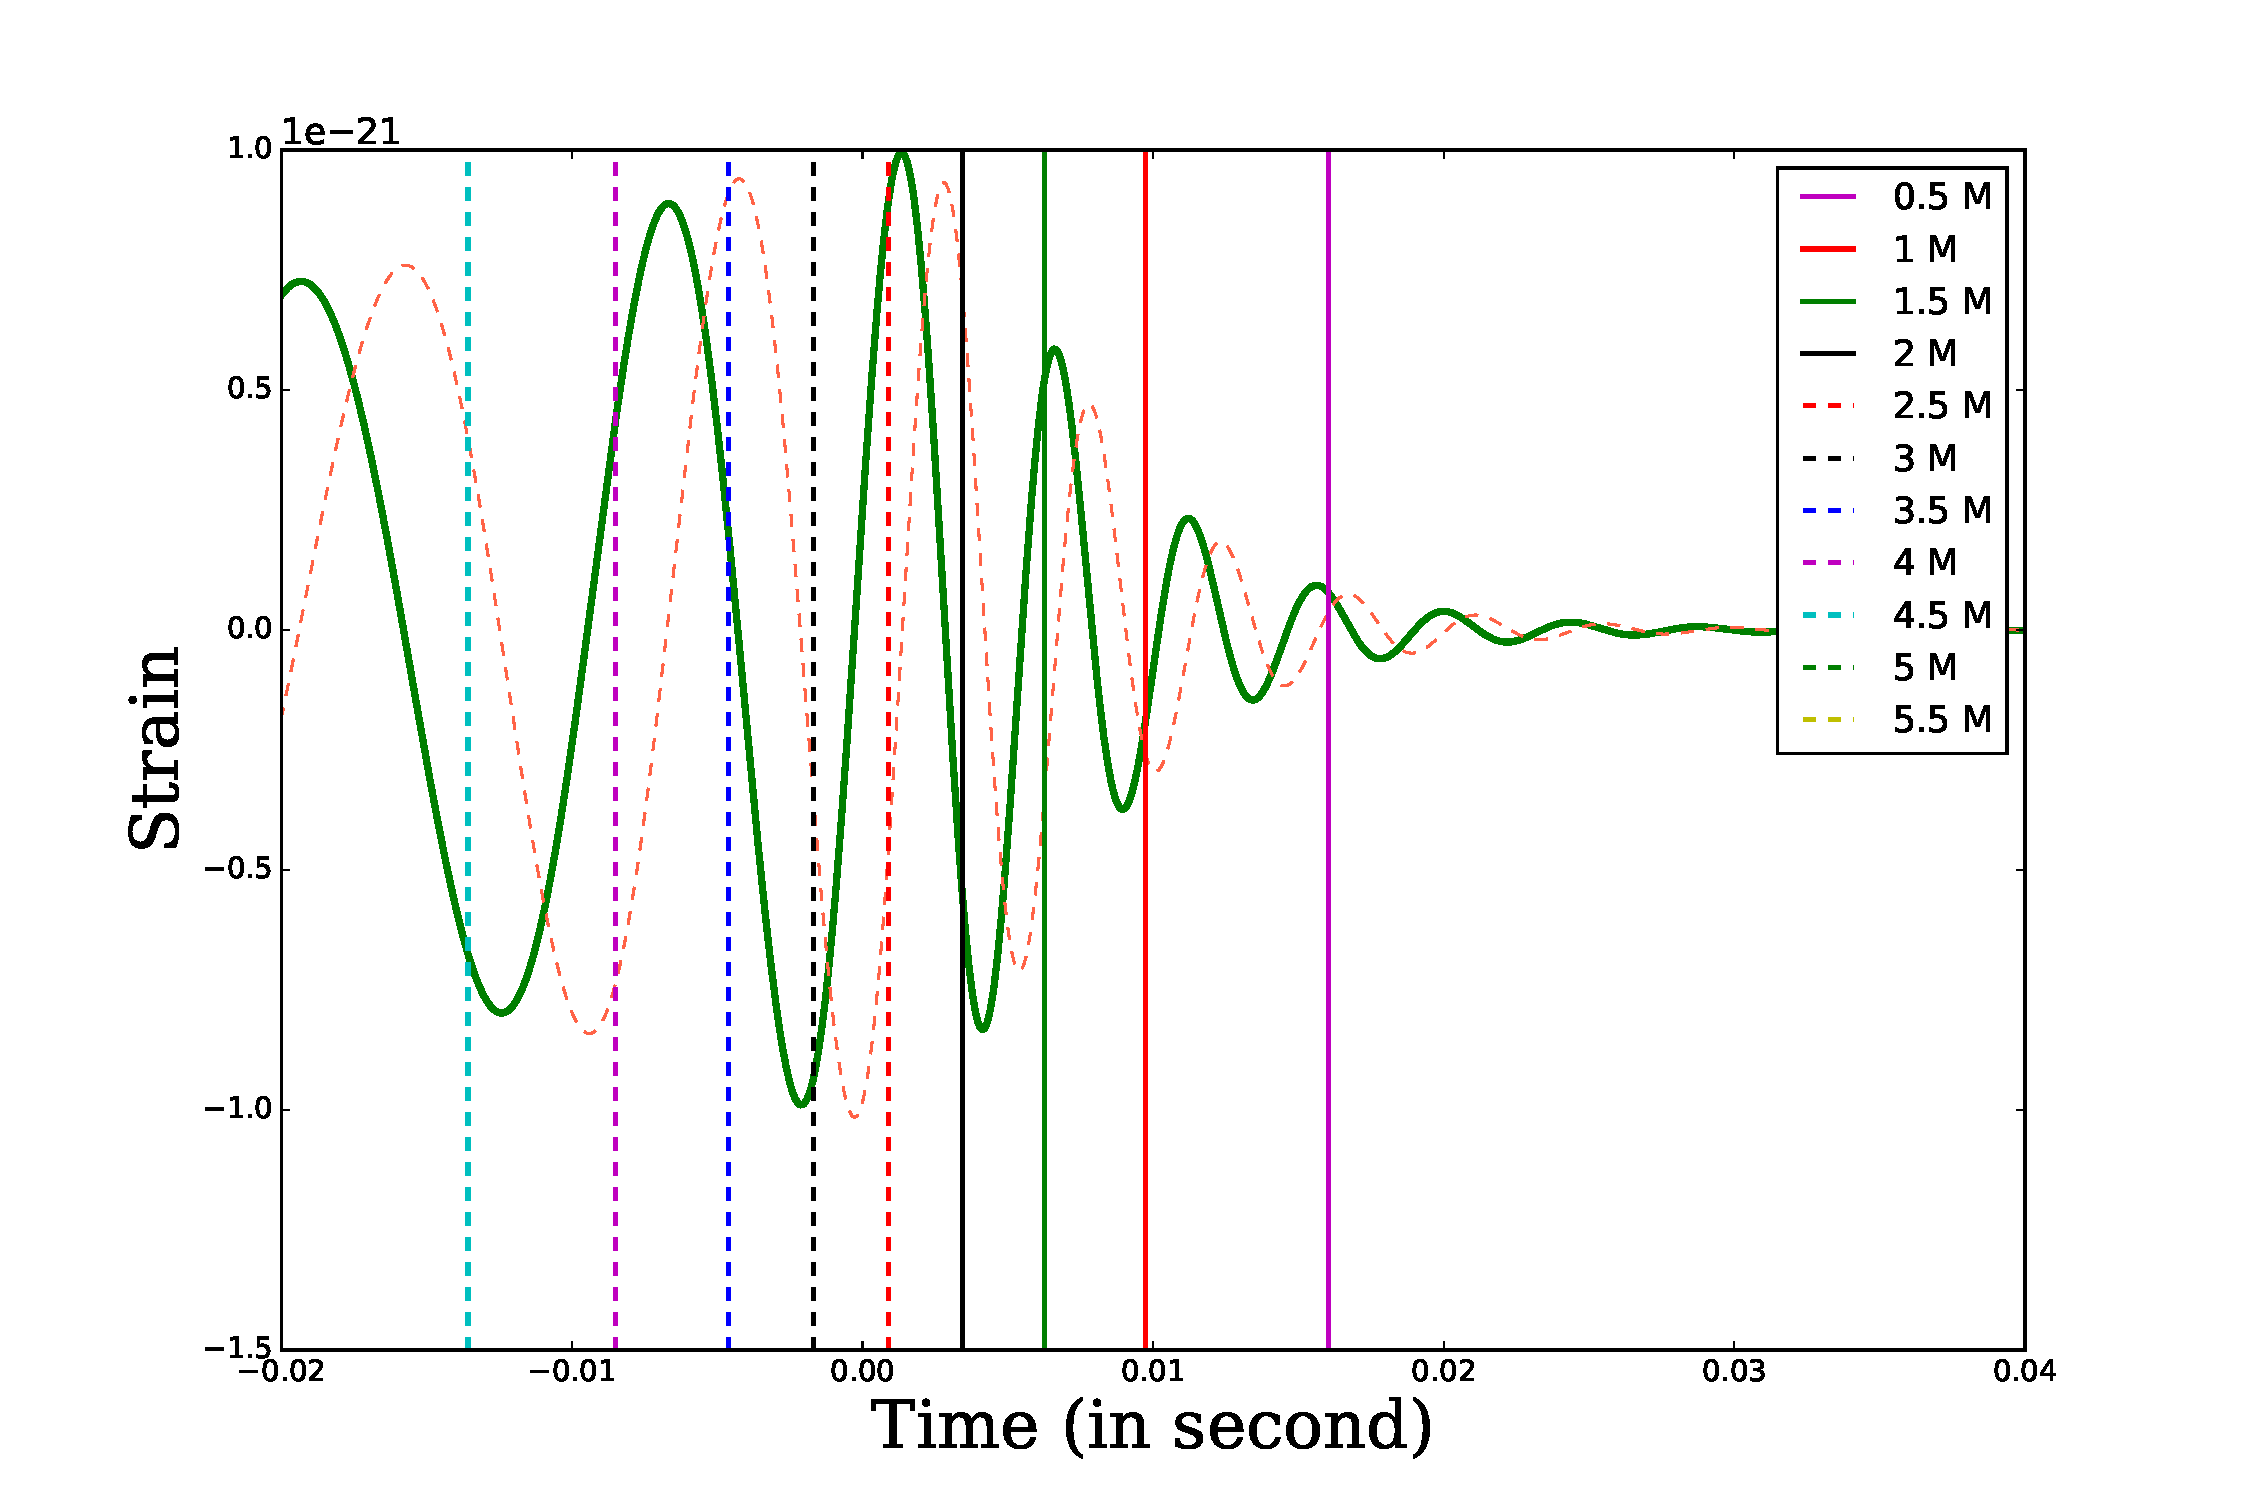
\includegraphics[width=0.8\textwidth]{figures/reffmarking.pdf}
\caption{$r_{\mathrm{eff}}$ marked on the GW strain. This plot presents the GW waveform corresponding to the best-fit template parameters reported by the PyCBC search pipeline for the event GW150914. The  waveform is zoomed in on the last few cycles. The lines indicate to the value of $r_{\mathrm{eff}}$ at different times of the evolution. The dotted lines correspond to separation vector before merger of the BBH system and the solid line correspond to un-physical separation, that provide the scale of perturbation in the merger-ringdown phase of the BBH evelotion. We use the units where $G = c = 1$. }
\label{fiig:reff_on_wave}
\end{figure}

We compute the evolution of deformation parameter $\delta << (t)$ for the waveform and present it in Figure \ref{fig:delta} which has the same time axis as figure \ref{fig:reff_on_wave}. For perturbation theory to hold $\delta \lle 1$. By comparing to Figure \ref{fig:delta} we can can infer that for analysis based on perturbation theory one should at least wait for roughly 0.005 ms after the peak of the waveform.  

\begin{figure}
\centering
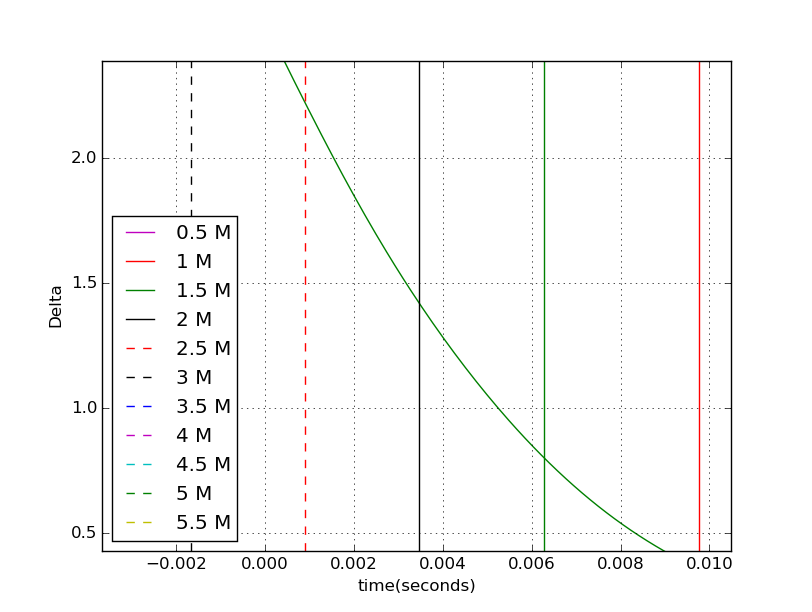
\includegraphics[width=0.8\textwidth]{figures/Delta_of_t.png}
\caption{Distortion parameter $\delta$ as a function of time. This plot shows the evolution of the distortion parameter $\delta$ defined in \ref{eq:deformation}. The scale of the pertrubation is comparable to the intrinsic scale of the system roughtly when $\delta =1 $. We see that about 0.005 sec after the peak of the waveform (which by convention is set at $t=0$, see figure \ref{fig:reff_on_wave}) the value of $\delta \sim 1$. A pertubation analysis should begin after this time.}
\label{fig:delta}
\end{figure}

Note that this is only approximate for the following reasons: First, both the models used are toy models, studied primarily with the intention of developing an intuition on the scale of perturbation. Second, in defining $\Delta$ we have used Schwarschild radius as the intrinsic scale of the system, whereas the final BH is a Kerr BH. In the next chapter, we will address the issue on the start time of ringdown in a rigorous way using a full numerical relativity evolution of the spacetime. 

